\subsection{One dimensional hydrogen chain}
We now move on to one of the simplest extended \emph{ab-initio} systems, a hydrogen chain with periodic boundary conditions. 
We consider the case of $10$ sites and work in a regime where 
inter-atomic distance is relatively large (1.5 to 3.0 \AA), 
such that the system is potentially well described by a 1-band Hubbard model (with primarily 
$s$-like orbitals, whose form we discuss). Since it is difficult to get exact many-body 
eigenstates, this example will highlight the utility of the N-AIDMD approach.

We first obtain single-particle Kohn-Sham orbitals from a set of spin-unrestricted and spin-restricted DFT-PBE calculations. 
With this set of orbitals, we produce a set of wavefunction states (\HHZ{Slater-Jastrow wave functions?}) 
consisting of singles- and doubles- excitations to the Slater determinant, %Allow $|KS \rangle $ to be the Slater determinant formed from the Kohn-Sham orbitals, and orbitals $i$ and $j$ ($k$ and $l$) to be Kohn-Sham orbitals that are unoccupied (occupied) in the Slater determinant. We then produce new wave function states as singles excitations $|s \rangle$ and doubles excitations $| d \rangle$ excitations to the Slater determinant:
\begin{subequations}
\begin{eqnarray}
| s \rangle = & \Big[a^\dagger_{i \sigma} a_{k \sigma}   | KS \rangle \Big]e^J \\
| d \rangle = & \: \Big[a^\dagger_{i \sigma} a^\dagger_{j \sigma'} a_{k \sigma'} c_{l \sigma}   | KS \rangle\Big]e^J ,
\end{eqnarray}
\end{subequations}
where $|KS\rangle$ is the Stater determinant of occupied Kohn-Sham orbitals, $\sigma$ and $\sigma'$ are spin indices, 
and $a_{i}^\dagger$ ($a_{i}$) is a single-electron creation (destruction) corresponding to Kohn-Sham orbitals, 
and $e^J$ is the Jastrow factor which was optimized using variational Monte Carlo. 

As described in section 2, the advantage of the N-AIDMD is that it does not need access the 
explicit eigenstates of the Hamiltonian, which allows many more states to be sampled in the process 
of characterizing the low-energy Hilbert of space of the system. The localized orbital basis upon which the descriptors are calculated 
is obtained by generating intrinsic atomic orbitals (IAO) from the Kohn-Sham orbitals, and orthogonalizing them using 
the L\"owdin procedure. \HHZ{Could you plot these orbitals and replace the Wannier orbitals stuff?}
These form the effective orbitals that enter the 1-band Hubbard Hamiltonian. 

Having computed the energies and descriptors for this set of wave functions, and verified the independence of the $U$ and $t$ descriptors, 
we fit a Hubbard-type model to describe the \textit{ab-initio} energetic results. 
Fig.~\ref{fig:RMS-Error-vs-Bond} shows the RMS error in the resultant $U$-$t$ model, relative to the \textit{ab-initio} DMC energetics, as a function of the hydrogen inter-atomic separation. 
We observe the the error is consistently less than 2 eV. The fitted value of the one-body hopping $t$ as a function of separation is shown in Fig.~\ref{fig:Parameters-vs-Bond-t}. 
As expected, the value of $t$ declines toward zero at larger separations. Hence, we see that the hydrogen chain can be well-described by a Hubbard-type model for a range of inter-atomic separations.

\begin{figure}
\centering
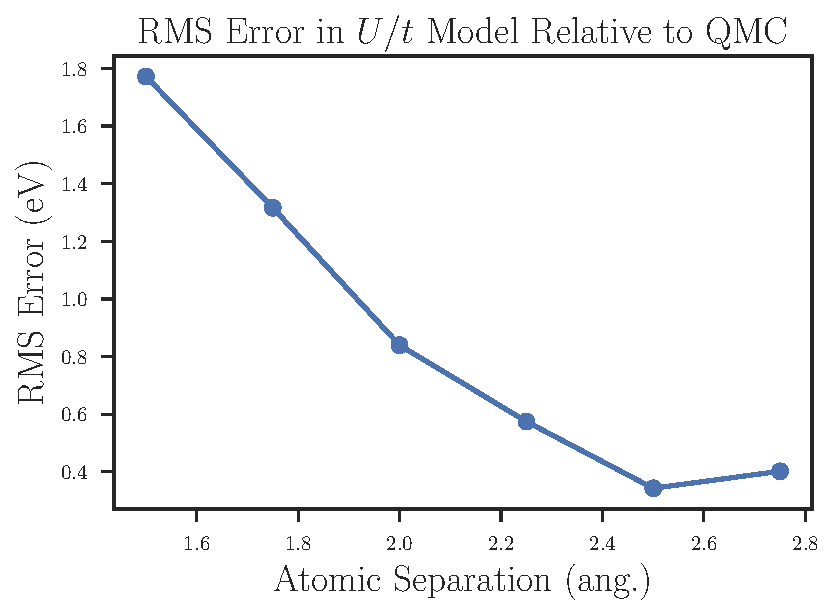
\includegraphics[scale=0.5]{./Figures/rms_ut_error_vs_separation_h_chain.pdf}
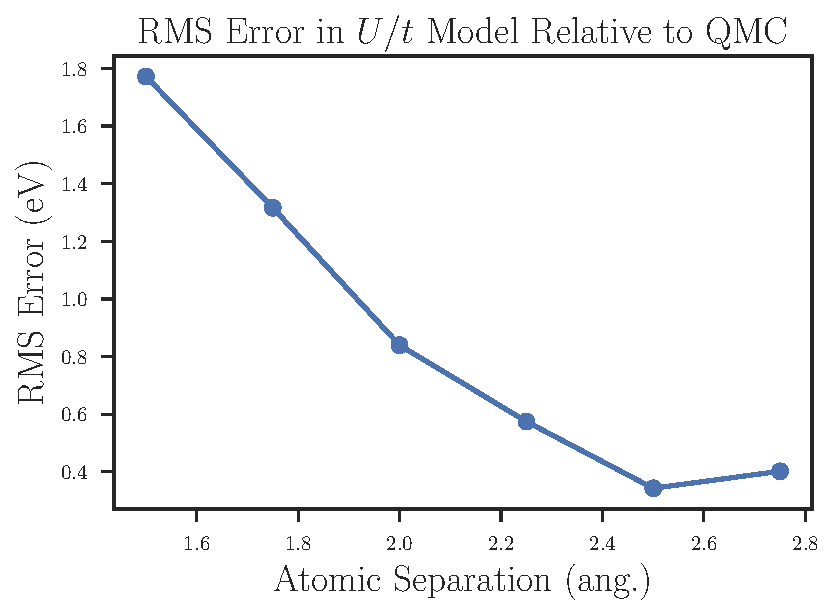
\includegraphics[scale=0.5]{./Figures/rms_ut_error_vs_separation_h_chain.pdf}
\caption{\HJC{Put model vs ab-initio plots here}The RMS error in the fitted $U$-$t$ model for the periodic H$_{10}$ chain, relative to the \textit{ab-initio} energies. The RMS error is less than 1 eV for sufficiently long bond lengths.}\label{fig:RMS-Error-vs-Bond}
\end{figure}
 
\begin{figure}
\centering
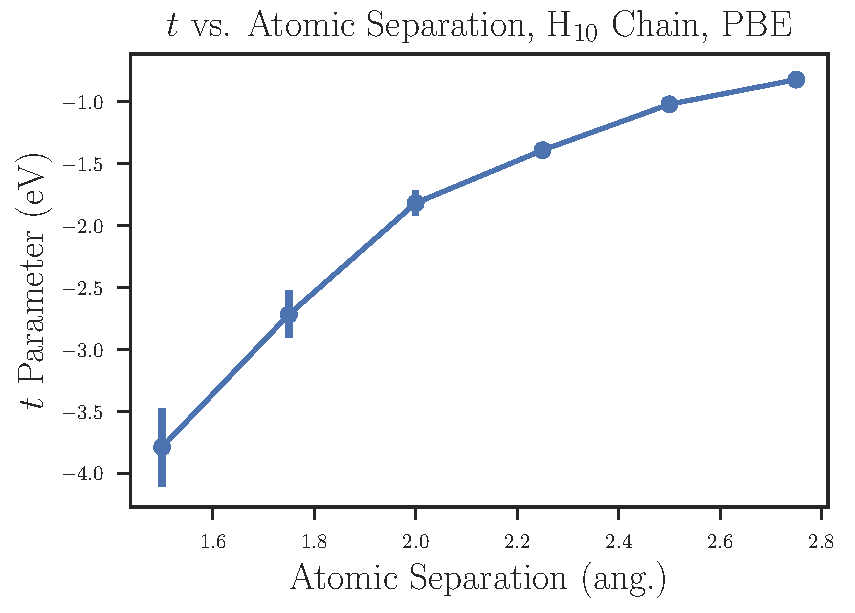
\includegraphics[scale=0.5]{./Figures/$t$_vs_separation_h_chain_ols.pdf}
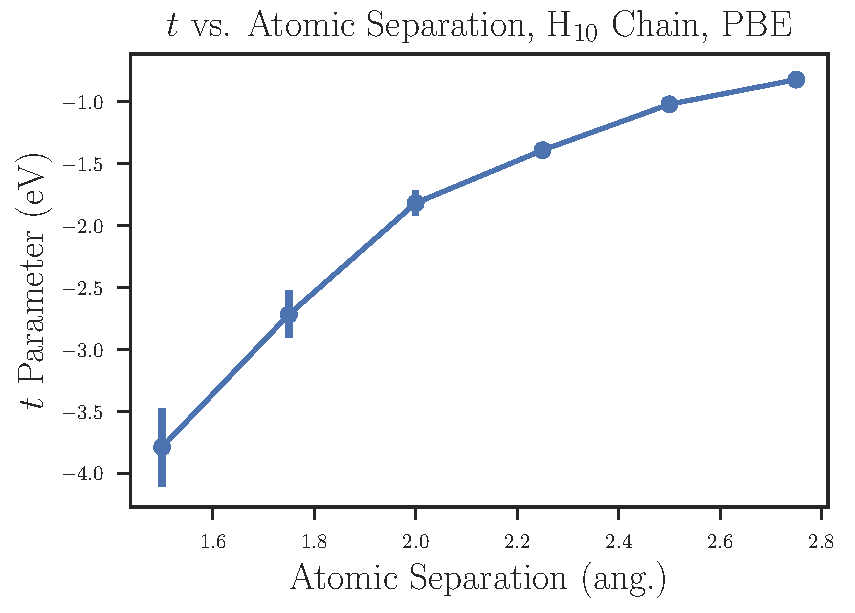
\includegraphics[scale=0.5]{./Figures/$t$_vs_separation_h_chain_ols.pdf}
\caption{\HJC{Put t vs r and U/t vs r} The one-body hopping $t$ parameter as a function of lattice constant for the periodic H$_{10}$ chain, obtained from a fitted $U$-$t$ model. The parameter value declines to zero as the lattice constant increases. \HHZ{I suggest to remove the titles from the figure, and put description in the caption instead. The y-axis label: how about "Hopping parameter $t$"}}\label{fig:Parameters-vs-Bond-t}
\end{figure}
